\section{Model}
In order to reliably reproduce experimental observations of dynein's step, a model of dynein should responsibly conserve dynein's spatial information and complex structure without limiting the physical interactions with its environment. Doing so computationally introduces a strict balance between model accuracy and computational efficiency. In an attempt to best satisfy this difficult balance, we propose a simple model of dynein under a series of assumptions that benefits quick simulations of dynein taking a step. 


\subsection{2D Rigid Rod Model}
Since our goal is to investigate dynein's interhead coordination during its forward directed stepping, we decided to model dynein as a 2-dimensional system of circular domains held together by massless rigid rods. These cirular domains embody the two binding domains, two motor domains, and one tail domain, where each domain act as independent angular springs with their own spring constants. A labeled picture of the model is shown below in Figure (\ref{fig:model}). 

\begin{figure}[H]
	\centering
	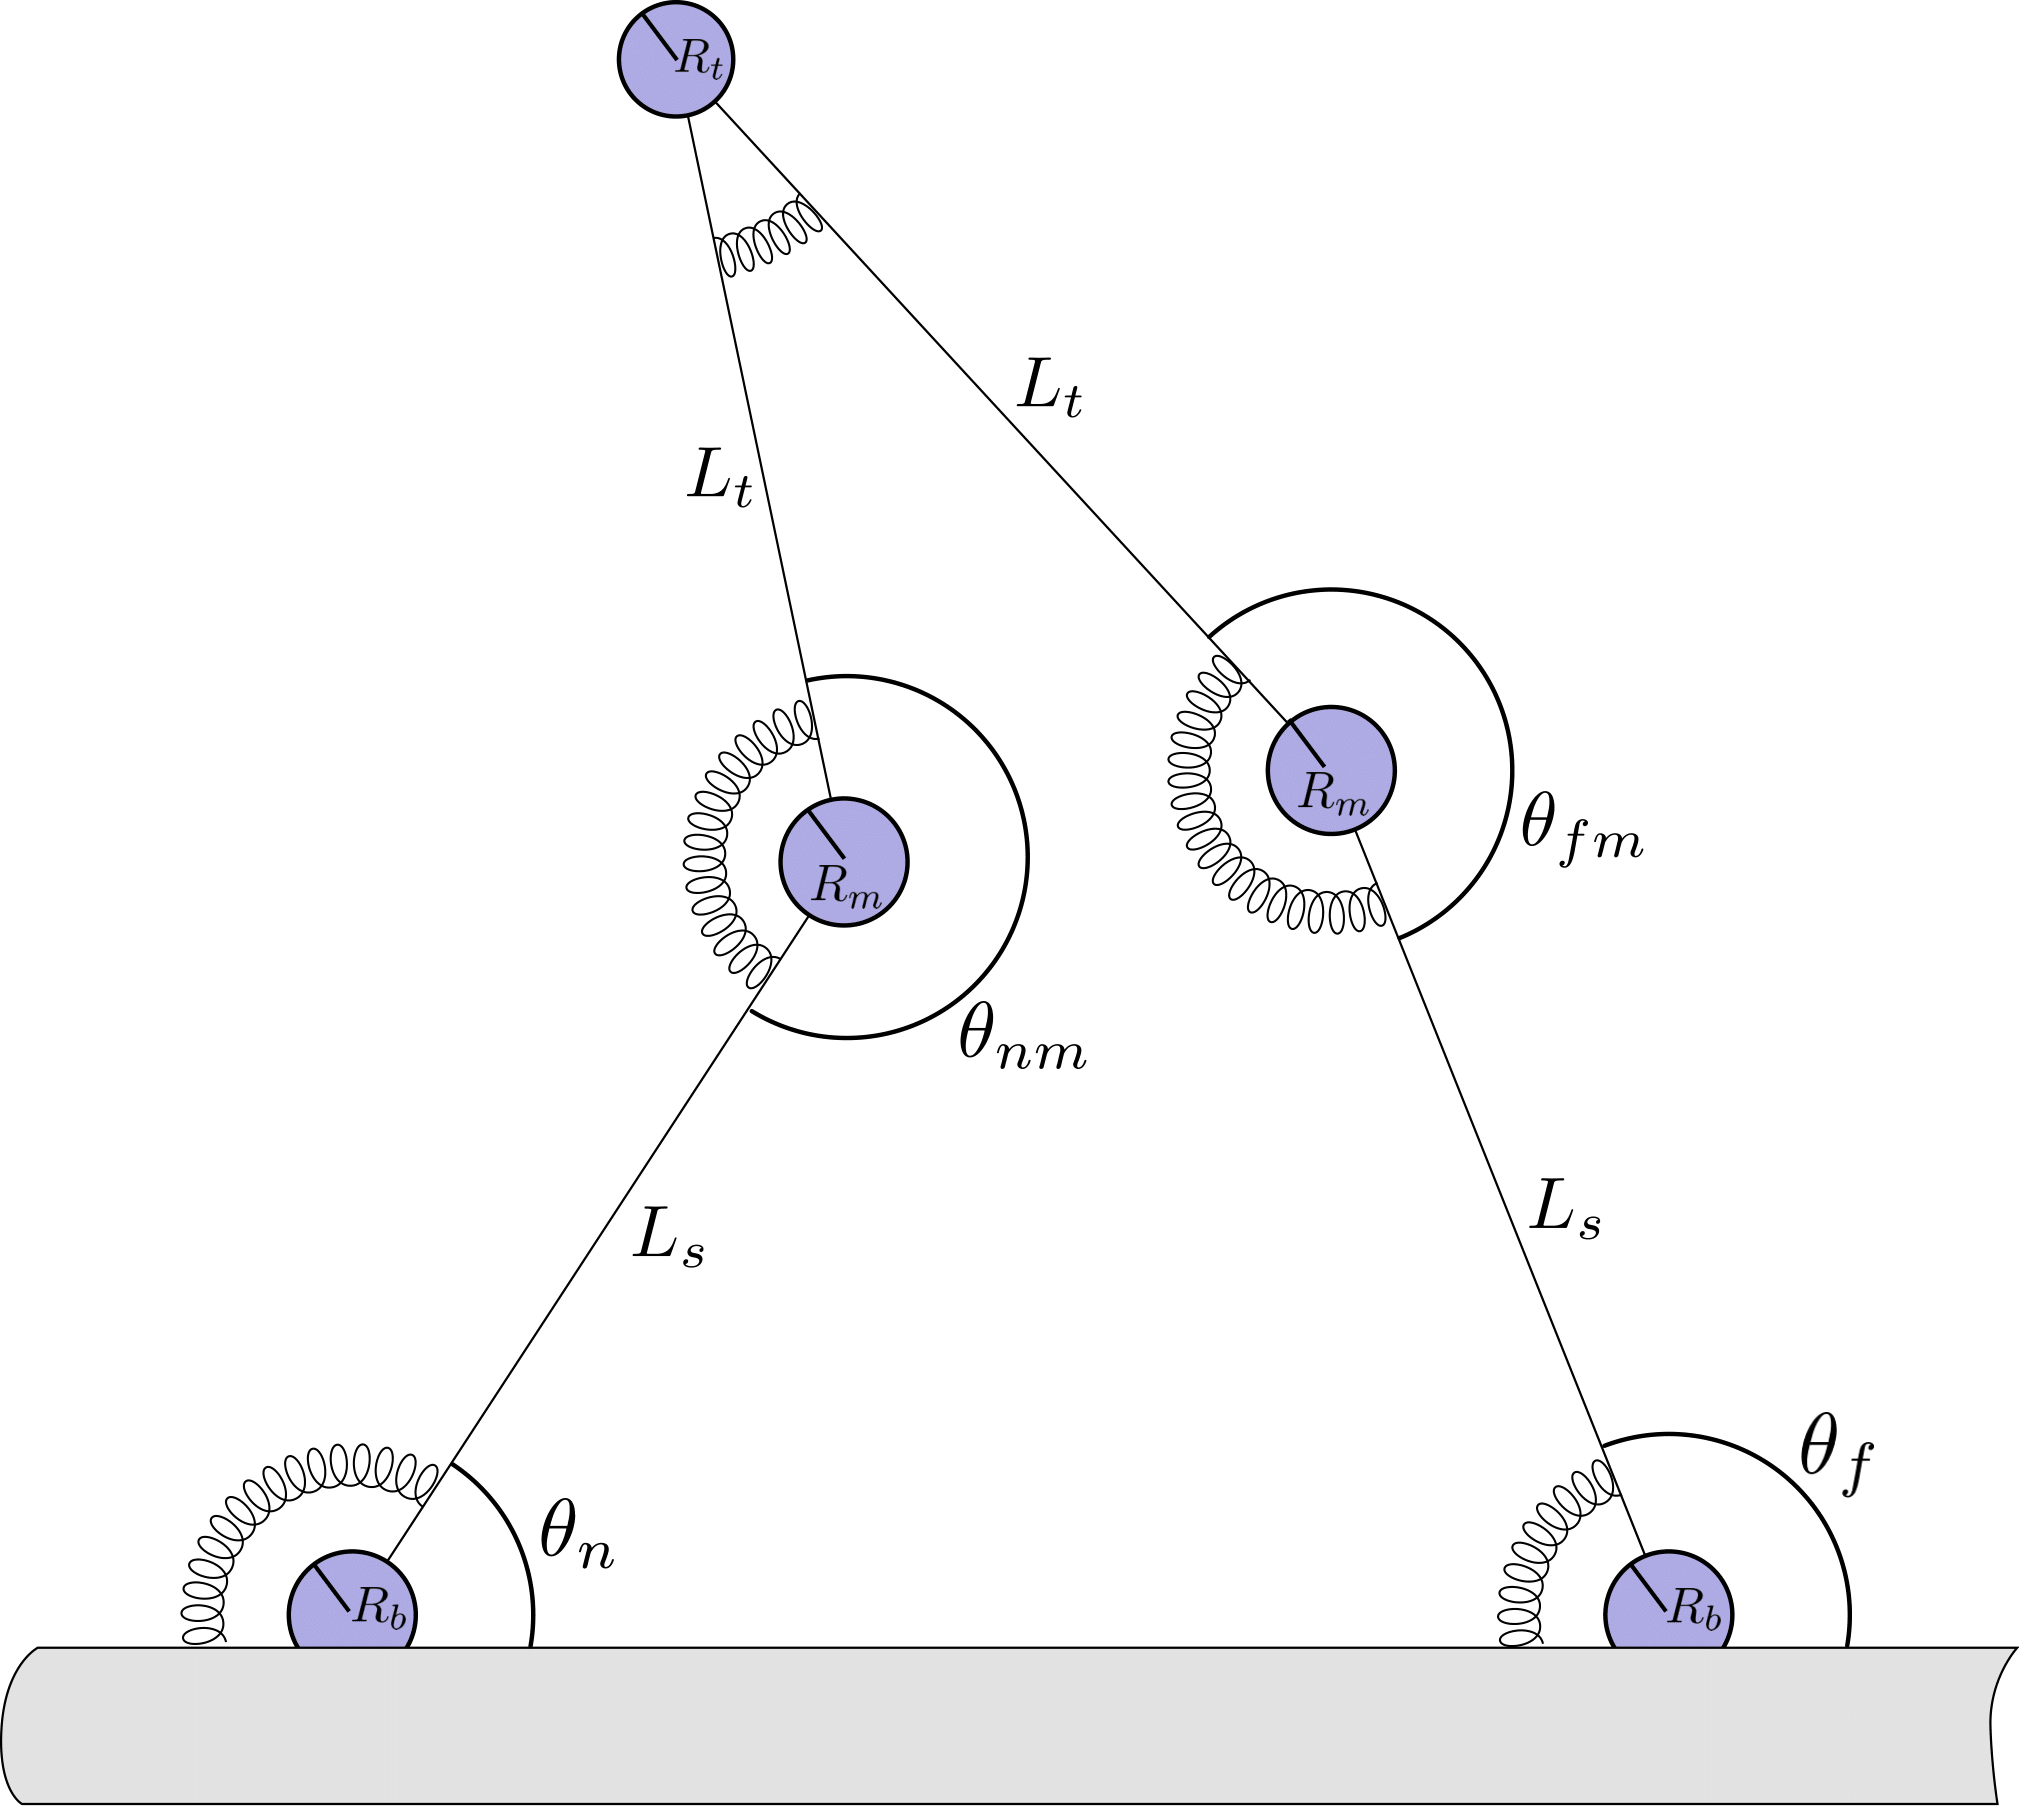
\includegraphics[width=0.6\columnwidth]{Figures/model-cartoon.png}
	\caption[Dynein Model]{\textbf{Dynein Model.} A model of the dynein in the both bound state where both binding domains are bounded to the microtubule. The springs are only a visualization of how they control the domains and are not a part of the model geometry. \cite{Capek2017}}
	\label{fig:model}
\end{figure}

Despite dynein's complexity allowing its step to vary in both length and direction, we limit our model to one direction to eliminate a dimension (the off-axis) when analyzing the forward stepping pattern of dynein. This would also simplify the asymmetry of the microtubule when the dynein is stepping either on the $\alpha$ or $\beta$ tubulin. We also simplify the stalk and linker to be massless because we are assuming the drag force to be much larger than the mass of the rods and domains. The reasoning for this will be later discussed in Section \ref{sec:BrownianDynamics} when we introduce Brownian dynamics. Although the stalk and linker of real dynein definitely have mass, we counteract the loss of interactions the rods experience with its environment by increasing the radii of the domains to be slightly larger than experimental measurements.

\subsection{Domains as Angular Springs}
In order to best simulate the stretching and forward kicking motion of the power stroke, we define our domains to act as springs with spring constants $c_b$, $c_m$, and $c_t$ -- one for each respective domain. This can be analogous to how humans walk as the domains are used as flexible joints when taking a step. Defining our domains as springs will also allow us to influence forward bias walking by introducing a restoring force in each domain using Hooke's law: 
\begin{equation}
    F_i=-c_i(\theta_i-\theta_{i,eq})
\end{equation}
where $c_i$ is the spring constant, $\theta_i$ is angle corresponding to the $i^{th}$ domain, and $\theta_{i,eq}$ is the equilibrium angle in which biases the motion. Using this, we can calculate the energy of each domain by integrating and arriving to the familiar equation for spring energy.
\begin{equation} \label{eq:energy}
    U_i=\frac{1}{2}c_i(\theta_i-\theta_{i,eq})^2
\end{equation}
%Since dynein is symmetric for each heavy chain leg, the equilibrium angle will be identical for both binding and motor domain pairs, i.e. $\theta_{b,eq}$ is defined as the equilibrium angle for both binding domains, while $\theta_{m,eq}$ is defined as the equilibrium angle for both motor domains. 
This equation would then be used throughout the entirety of the simulation to determine the total energy of our dynein at a given conformation. 


\subsection{Two-State System}
According to the Mechanochemical Cycle (Figure \ref{fig:MechanochemicalCycle}), dynein can be in eight states over the course of a single step. However, many of these states possess similar conformations, where the dynein either has one binding domain bounded while the other diffuses above the microtubule or has both binding domains bounded to the microtubule. Since we assume simple ATP exchange and that the two physical states are during binding and unbinding \cite{}, we categorize the cycle into two main conformations: the pre-stroke one bound state and the post-stroke both bound state.

\begin{figure}[H]
	\centering
	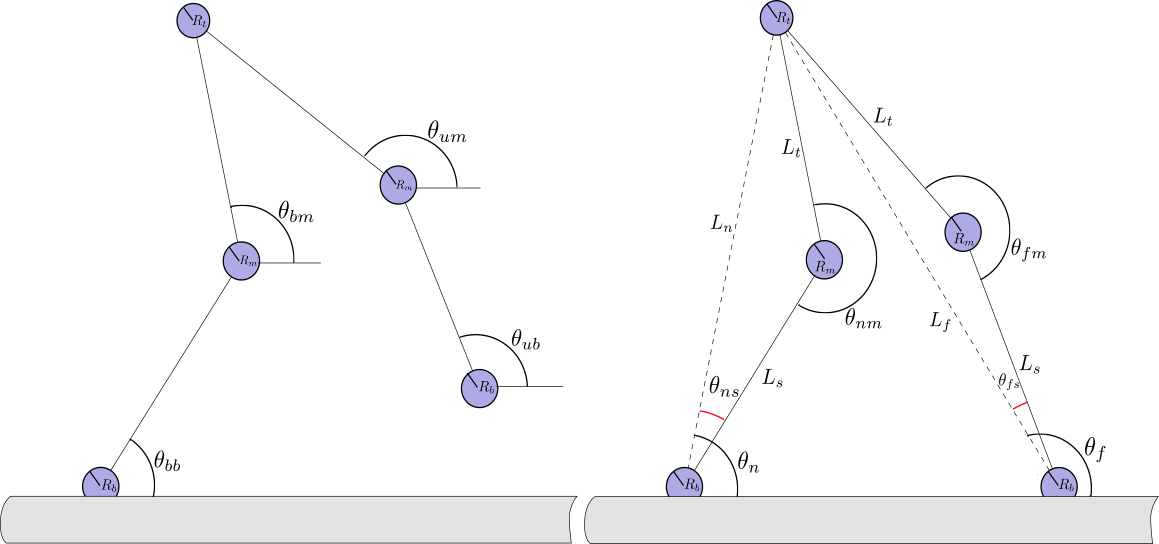
\includegraphics[width=0.9\columnwidth]{Figures/OB_vs_BB.PNG}
	\caption[One Bound vs. Both Bound]{\textbf{One Bound vs. Both Bound} \textit{Figure on left}: Prestroke one bound state with labeling scheme 'b-’ and ‘u-’ for bound leg and unbound leg. \textit{Figure on the right}: Poststroke both bound state with labeling scheme ‘n-’ and ‘f-’ for ``near" leg and ``far'' leg. \cite{Capek2017}.}
	\label{fig:OBvsBB}
\end{figure}

Differentiating the two allows us to more conveniently bias the conformational change by defining different equilibrium angles for both states. Since dynein is symmetric for each heavy chain leg, the equilibrium angles for the both bound state will be identical for both binding and motor domain pairs, i.e. $\theta_{b,eq}$ is defined as the equilibrium angle for both binding domains, while $\theta_{m,eq}$ is defined as the equilibrium angle for both motor domains. However, in the one bound state, the unbound leg wants to exhibit the powerstroke and kick out. Therefore, the equilibrium angles for the motor domains will differ in order to bias the unbound leg to straighten and perform the powerstroke. 


\subsection{Transitioning Between States}
%\textit{Physics about conformational energy changes. How we model transitioning between BB state and OB state using transitioning rates and spring energies.}

Similar to other simulations, the binding and unbinding process will be governed by a rate-limiting step, where each process will be associated with binding rates. These binding rates will be model parameters defined by binding constants with units of probability per time. When the dynein is in the one bound state, we assume that the unbound binding domain can only bind when it is within a vertical range of the microtubule, i.e.
\begin{equation}
	\rho_b=k_b(1-H(r_{ub,y}-\epsilon)).
\end{equation} 
Here, the $\rho_b$ is the binding rate, $k_b$ is the rate constant, $H$ is the Heaviside step function, $r_{ub,y}$ is the y position of the unbound binding domain, and $\epsilon$ is the range within the microtubule.

When the dynein is in the both bound state and wants to unbind, we incorporate a stepping bias in the unbinding rate. As supported from Yildiz in Figure (\ref{fig:trailingbias}), the likelihood of the trailing leg unbinding is greater than the leading leg when the distance between the two legs increase. 


\begin{figure}[H]
	\centering
	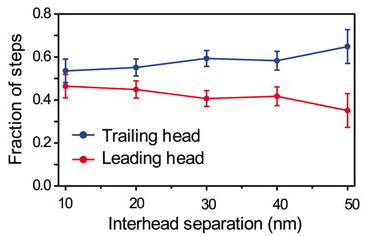
\includegraphics[width=0.6\columnwidth]{Figures/trailingbias.png}
	\caption[Probability of Unbinding Bias]{\textbf{Probability of Unbinding Bias.} The probability of either trailing or leading steps which correspond to the model's ``near" or ``far" leg unbinding, respectively. \cite{Dewitt2012}.}
	\label{fig:trailingbias}
\end{figure}

To favor trailing steps, we define an angle dependent exponential factor within the binding domains and mathematically express this as,
\begin{equation}
	\rho_{ub}=k_{ub}e^{C(\theta_b-theta_{b,eq})}.
\end{equation}
We introduce a new model parameter $C$, the exponential unbinding constant, that allows us to control this bias. For the trailing step bias we want to achieve, we define $C$ to be negative because the trailing $\theta_b$ tends to be less than the leading $\theta_b$ and  when $\theta_b$ is less than $\theta_{b,eq}$, the unbinding rate becomes large.


\section{Simulation}

The key difference between the works discussed in \cite{Capek2017, } (\textit{Elliott and John's paper}) and this paper is the implementation of a Monte Carlo algorithm in replacement for the Brownian dynamics both bound state. Capek and Waczak were able to fully simulate both states of dynein's walk with a Brownian dynamics simulation and collect data of multiple steps during a walk. However, they noticed that their simulation took significant computation time because of the unbinding process taking a large amount of time relative to the total stepping time. They also noticed that the both bound configuration of dynein does not impact the final step length. We developed this new method of analyzing the both bound state to significantly improve computational efficiency while still maintaining the dynamical simulation of the actual step in the one bound state. 

%These quick simulations are governed by a Monte Carlo algorithm, while the movement of the model is dictated by equations of motion describing domains interacting with a force of drag and a random force. This type of molecular simulations are more commonly known as Brownian dynamics. (\textbf{Possible take out sentence introducing MC and Brownian dynamics for later})


\subsection{Brownian Dynamics for One Bound}
\label{sec:BrownianDynamics}

When simulating dynein's one bound motion, the domains of constant mass must still obey classical Newtonian physics and follow Newton's laws of motion. Knowing this, we can use Newton's second law to derive the equations of motion for each domain when experiencing various forces. That is,
\begin{equation}
	\sum_{i}\textbf{F}_i=m\ddot{\textbf{r}}.
\end{equation} 

For our domains experiencing the aqueous environment in the cell, the first force we can identify is the force of linear drag:
\begin{equation}
	\textbf{F}_{drag}=-\gamma \dot{\textbf{r}}
\end{equation}
where $\gamma$ is the drag coefficient defined from Stokes' law to be:
\begin{equation}
	\gamma=6\pi\eta a.
\end{equation}
This equation specifies the drag term by a given radius $a$ and liquid viscocity $\eta$. 

The secondary force that we can easily identify is the random force inspiring the Brownian motion. This force describes the random interactions the domains experience with the paticles making the solvent and will be denoted as \textbf{F}$_{rand}$. The ``randomness" will be sampled from a zero-centered Gaussian with variance:
\begin{equation}
	\sigma^2=\sqrt{\frac{2\gamma}{\beta\Delta t}}.
\end{equation}
where $\beta$ is the thermodynamic beta and $\Delta t$ is a time-step. 

The final existing force on the domains will be the tension force the domains have on each other \textit{via} their connecting rods. We will name this \textbf{F}$_T$. Incorporting all these forces with Newton's second law, we can produce an equation otherwise known as the \textit{Langevin Equation}:
\begin{equation}
	-\gamma \dot{\textbf{r}} + \textbf{F}_{rand} + \textbf{F}_T = m\ddot{\textbf{r}}.
\end{equation}
As mentioned earlier, in order to properly demonstrate Brownian dynamics, we must assume strong drag where $|\gamma \dot{\textbf{r}}|\ll |m\ddot{\textbf{r}}|$. Or in otherwords, we assume that the immense viscosity in the environment stricts the ability for our domains to accelerate. Simplifying the \textit{Langevin Equation} and solving for $\dot{\textbf{r}}$, we get:
\begin{equation}
	\dot{\textbf{r}}=\frac{1}{\gamma}(\textbf{F}_{rand} + \textbf{F}_T)
\end{equation}
which is a differential equation we can solve for the equations of motion for the domains in the one bound state. The derivation and final equations of motion can be found in \cite{Capek2017, W}


\subsection{Monte Carlo Algorithm}
Since research and Waczak/Capek suggests that the dynein spends the majority of the stepping time in the both bound state, we can safely assume that the dynein equilibriates before unbinding. This allows us to use Monte Carlo methods for analyzing a single step by interpreting our model as a system. Typically, Monte Carlo methods are used to analyze equilibrium theromodynamics of fluids where a system of atoms can possess many different microstates. For this model, the dynein is the system and the different possible microstates are the both bound configurations our model can achieve. Each both bound configuration are independent from one another and can produce different total energy values. The benefit of this method is the ability to sample a large ensemble of both bound states and quickly generate statitics about the step. Eventually, this will allow us to create probability distributions for important variables. The algorithm is as follows:
\begin{algorithm}[H]
	\caption{Monte Carlo}
	\label{alg:MonteCarlo}

	\begin{alg}
	\item Initialize an unsigned distance, L, between the binding domains.
	
	\item Randomly pick 4 angles ($\theta_0$, $\theta_1$, $\theta_2$, $\theta_3$) to generate a completely random configuration of dynein in space. (\textit{Include picture})
	
	\item Calculate the distance between the binding domains and check if the distance is within a range of $L\pm l$, where $l$ is arbitrarily small.
	
	\item Rotate the configuration so that both binding domains are on the microtubule and recalculate both bound state angles with the naming convention in Figure (\ref{fig:OBvsBB}).
	
	\item Calculate the total energy of the configuration by summing the energy of each domain (using Equation (\ref{eq:energy})).
	\begin{equation}
		E_{total, n}=\sum_{i}\frac{1}{2}c_i(\theta_i-\theta_{i,eq})^2
	\end{equation}
	Here, $n$ refers to the specific both bound configuration.	
	
	\item Define a Boltzmann distribution for the relative probability of unbinding and a partition function, $Z$.
	\begin{equation}
		P_{ub}\propto e^{-\beta E_{total, n}}
	\end{equation}
	\begin{equation}
		Z=\sum_{n}e^{\beta E_{total, n}}
	\end{equation}
	
	\item Calculate the probability of unbinding with the unbinding rate and Boltzmann distribution.
	\begin{equation}
		P_{ub} = \rho_{ub}e^{-\beta E_{total, n}}
	\end{equation}
	
	\item ``Roll a die" for a value within the range of $[0,1]$ and check if the value is less than $P_{ub}$. If not, repeat algorithm from step 1.
	
	\item If dynein unbinds, run one bound Brownian dynamics simulation of the step and wait until rebinding.
	
	\item Collect statistics about final displacement and one bound time. 	
	
	\end{alg}

\end{algorithm}

 



%\textit{STRAIGHT FROM PROPOSAL. FIXME}

%Our entire model of dynein will be coded with a combination of both Python and C++. The structural features of dynein will be captured with a two-dimensional geometric model of circular domains connected by rigid rods. The dynamics of dynein will be captured by imposing both equilibrium and Brownian forces on each circular domain of the model, while the chemical properties will be modeled by sporadically transitioning between two states: a poststroke both bound state, and a prestroke one bound state. These two states are shown below in Figure 2.
%
%The simulation for stepping will consist of running multiple independent steps that starts in a both bound configuration and transitions into the Brownian dynamics one bound state. In this state, each domain will undergo Brownian forces until the unbounded leg diffuses back onto the microtubule, thus completing a step. The Brownian dynamics only affects the one bound state since that is the only time (in our model) the domains undergo molecular interaction with its surroundings to achieve processive motion. This Monte Carlo method of collecting an ensemble of statistics after many simulations will lead to probability distributions of measured variables that can be compared with experimental results. The common experimental results analyzed in this field are the distribution of step lengths (defined as the final displacement of the “stepping” leg minus the initial displacement), stepping times, probability of the binding domain unbinding, and the velocity of a step. Once sufficient data is collected for each listed variable, plotting scripts on Python will be used to visualize the possible relationships between these variables and generate analysis for our model’s stepping patterns. Currently, a paper published by Dr. Ahmet Yildiz from the University of Berkeley proposed a possible relationship within dynein’s stepping, implying inter-step correlation [3]. Our model aims to reproduce these results by finding a set of parameters that matches Yildiz’s observation in the form of a linear regression of the step lengths against the initial binding domain separation. We hope to either support Yildiz’s claim or infer some new property of dynein that generated Yildiz’s observation.